\section{Evaluation}
\label{flexheap:sec:eval}

\subsection{Performance Compared to GC-Based Resizing Mechanisms}
Figure~\ref{fig:es_g1_throughput} depicts ingestion and search throughput for Elasticsearch under G1-50 and \flexheapName{}, corresponding to the first and third bars in each group.
The results are normalized to G1-50 (higher is better).
\flexheapName{} improves ingestion throughput by 5--20\% over G1-50 by allowing more DRAM to flow to the heap during ingestion phases with high allocation pressure, which reduces GC frequency and avoids full GCs caused by the 50\% cap.
For example, in the Wikipedia workload with an \SI{8}{GB} DRAM budget, G1-50 incurs 17 full GCs during ingestion whereas \flexheapName{} incurs none.
\flexheapName{} also improves search throughput by up to $7\times$, driven by lower device I/O, with read traffic reduced by up to 30\% in the dense vector workload, as shown in Table~\ref{tab:es_traffic}.
For example, in the Wikipedia workload the average I/O wait falls from 23\% (G1-50) to 17\% with \flexheapName{}, allowing the I/O cache to serve more requests and sustain a higher query rate.

\begin{figure*}[t]
	
\includegraphics[width=0.25\linewidth]{flexheap/fig/eval/es_g1_fh_legend.pdf}
	\\
	\subfloat[Wikipedia]{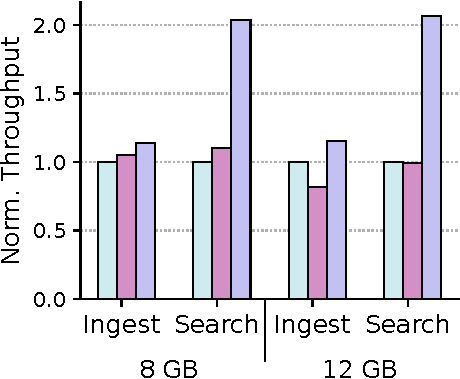
\includegraphics[width=0.245\linewidth]{flexheap/fig/eval/es_wiki.pdf}}
	\subfloat[Cohere Vector]{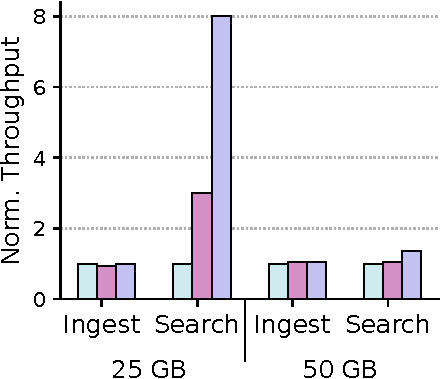
\includegraphics[width=0.245\linewidth]{flexheap/fig/eval/es_cv.pdf}}
	\subfloat[Dense Vector]{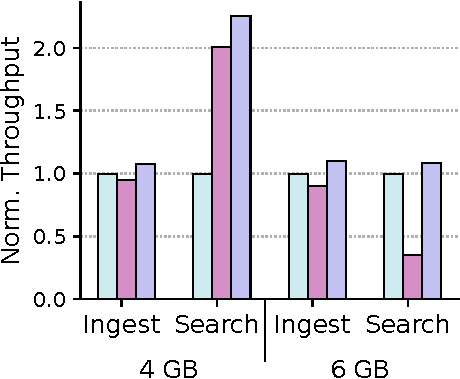
\includegraphics[width=0.245\linewidth]{flexheap/fig/eval/es_dv.pdf}}
	\subfloat[OpenAI Vector]{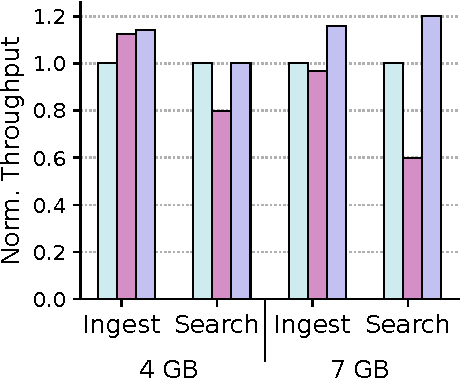
\includegraphics[width=0.245\linewidth]{flexheap/fig/eval/es_ai.pdf}}
	\caption{Ingestion and search throughput for Elasticsearch workloads under
		G1-50 (maximum heap cap of 50\% of DRAM), VG1, and \flexheapName{}.}
	\label{fig:es_g1_throughput}
\end{figure*}

% \begin{table}[t]
% 	\caption{Read and write I/O traffic for Elasticsearch workloads under G1-50
% 		and \flexheapName{} (FH) in small DRAM budget configurations.}
% 	\label{tab:es_traffic}
% 	\resizebox{0.5\columnwidth}{!}{%
% 		\begin{tabular}{llll|lll}
% 			              & \multicolumn{3}{c|}{\textbf{Read Traffic}} & \multicolumn{3}{c}{\textbf{Write Traffic}}                                                                                                                                                   \\
% 			              & \multicolumn{1}{c}{\textbf{G1-50}}         & \multicolumn{1}{c}{\textbf{FH}}            & \multicolumn{1}{c|}{\textbf{Diff}} & \multicolumn{1}{c}{\textbf{G1-50}} & \multicolumn{1}{c}{\textbf{FH}}   & \multicolumn{1}{c}{\textbf{Diff}} \\
% 			              & \multicolumn{1}{c}{\textbf{(GB)}}          & \multicolumn{1}{c}{\textbf{(GB)}}          & \multicolumn{1}{c|}{\textbf{(\%)}} & \multicolumn{1}{c}{\textbf{(GB)}}  & \multicolumn{1}{c}{\textbf{(GB)}} & \multicolumn{1}{c}{\textbf{(\%)}} \\ \hline
% 			Wikipedia     & 1677                                       & 1444                                       & \textbf{-14\%}                     & 637                                & 605                               & \textbf{-5\%}                     \\
% 			Cohere Vector & 29862                                      & 23636                                      & \textbf{-21\%}                     & 331                                & 334                               & +0.9\%                            \\
% 			Dense Vector  & 189                                        & 134                                        & \textbf{-29\%}                     & 79                                 & 85                                & +7\%                              \\
% 			OpenAi        & 716                                        & 638                                        & \textbf{-10\%}                     & 467                                & 432                               & \textbf{-7\%}                     \\ \hline
% 		\end{tabular}
% 	}
% \end{table}

\begin{table}[t]
	\caption{Read and write I/O traffic for Elasticsearch workloads under G1-50 (maximum heap cap
		of 50\% of DRAM), VG1, and \flexheapName{} (FH) in small DRAM budget configurations.}
	\label{tab:es_traffic}
	\resizebox{\columnwidth}{!}{%
		\begin{tabular}{l|ccccc|ccccc}
			\toprule
			              & \multicolumn{5}{c|}{\textbf{Read Traffic}} & \multicolumn{5}{c}{\textbf{Write Traffic}}                                                                                                                                                          \\
			\cmidrule(lr){2-6} \cmidrule(lr){7-11}
			              & \textbf{G1-50}                             & \textbf{VG1}                               & \textbf{FH}   & \textbf{Diff}        & \textbf{Diff}      & \textbf{G1-50} & \textbf{VG1}  & \textbf{FH}   & \textbf{Diff}        & \textbf{Diff}      \\
			              & \textbf{(GB)}                              & \textbf{(GB)}                              & \textbf{(GB)} & \textbf{FH vs G1-50} & \textbf{FH vs VG1} & \textbf{(GB)}  & \textbf{(GB)} & \textbf{(GB)} & \textbf{FH vs G1-50} & \textbf{FH vs VG1} \\
			\midrule
			Wikipedia     & 1677                                       & 3442                                       & 1444          & \textbf{-14\%}       & \textbf{-57\%}     & 637            & 587           & 605           & \textbf{-5\%}        & +3\%               \\
			Cohere Vector & 29862                                      & 27100                                      & 23636         & \textbf{-21\%}       & \textbf{-13\%}     & 331            & 336           & 334           & +0.9\%               & \textbf{-0.6\%}    \\
			Dense Vector  & 189                                        & 468                                        & 134           & \textbf{-29\%}       & \textbf{-71\%}     & 79             & 79            & 85            & +7\%                 & +7\%               \\
			OpenAI        & 716                                        & 700                                        & 638           & \textbf{-10\%}       & \textbf{-8\%}      & 467            & 435           & 432           & \textbf{-7\%}        & \textbf{-0.7\%}    \\
			\bottomrule
		\end{tabular}
	}
\end{table}


Next, we evaluate \flexheapName{} against G1 in Spark.
Figures~\ref{fig:spark_g1}(a) and \ref{fig:spark_g1}(b) report per-query speedups on TPC-DS with \SI{16}{\giga\byte} and \SI{32}{\giga\byte} DRAM budgets.
\flexheapName{} delivers more than 10\% speedups on roughly 40\% of queries with a \SI{16}{\giga\byte} DRAM budget and on 27\% of queries with \SI{32}{\giga\byte}.
The gains are smaller at \SI{32}{\giga\byte} because the larger DRAM budget leaves a larger I/O cache even under G1, reducing the headroom for \flexheapName{} to improve I/O performance.
The gains correlate with lower device pressure: read I/O drops by up to 30\%, because \flexheapName{} reassigns DRAM from the heap to the I/O cache during I/O-intensive phases and grows the heap when allocation pressure rises.
As a concrete example highlighted in Figures~\ref{fig:spark_g1}(c) and (d), q28 improves by 50\% when \flexheapName{} maintains a smaller committed heap throughout the run, which preserves a larger I/O cache and cuts average I/O wait by about 30\%.
For queries where \flexheapName{} matches G1, the traces show little or no I/O bottleneck, so I/O cache size is not the limiting factor and both mechanisms exhibit similar I/O traffic.

\begin{figure*}[h]
	
\includegraphics[width=0.6\linewidth]{flexheap/fig/eval/spark/analysis/legend.pdf}
	\\
	\subfloat[16\:GB]{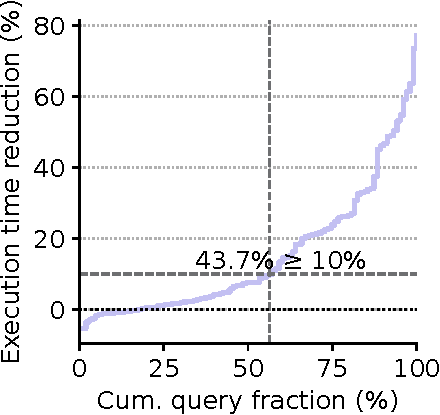
\includegraphics[width=0.24\linewidth]{flexheap/fig/eval/spark/tpcds_g1_fh.pdf}}
	\subfloat[32\:GB]{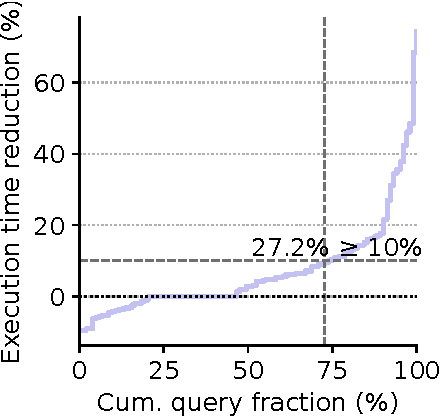
\includegraphics[width=0.24\linewidth]{flexheap/fig/eval/spark/tpcds_g1_fh_32g.pdf}}
	\subfloat[Q28-G1]{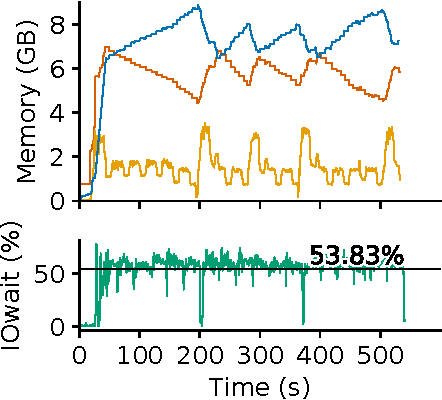
\includegraphics[width=0.24\linewidth]{flexheap/fig/eval/spark/analysis/q28_g1_10g_16g.pdf}}
	\subfloat[Q28-FlexHeap]{\includegraphics[width=0.24\linewidth]{flexheap/fig/eval/spark/analysis/q28_fh_10g_16g.pdf}}
	\caption{Performance improvement of \flexheapName{} over G1-75 (maximum heap cap 75\% of
		DRAM) heap resizing in Spark-SQL on TPC-DS.}
	\label{fig:spark_g1}
\end{figure*}

% \begin{figure*}[h]
% 	
\includegraphics[width=0.5\linewidth]{flexheap/fig/eval/spark/analysis/legend.pdf}
% 	\\
% 	\subfloat[Q28-G1]{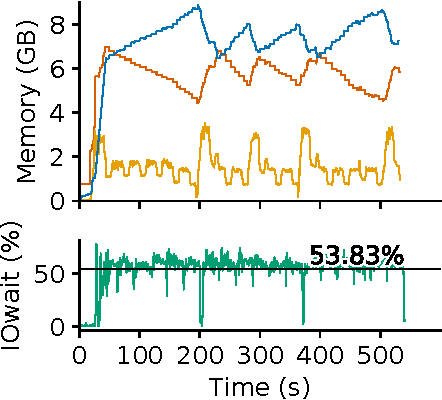
\includegraphics[width=0.24\linewidth]{flexheap/fig/eval/spark/analysis/q28_g1_10g_16g.pdf}}
% 	\subfloat[Q28-FH]{\includegraphics[width=0.24\linewidth]{flexheap/fig/eval/spark/analysis//q28_fh_10g_16g.pdf}}
% 	\subfloat[Q66-G1]{\includegraphics[width=0.24\linewidth]{flexheap/fig/eval/spark/analysis/q66_g1_10g_16g.pdf}}
% 	\subfloat[Q66-FH]{\includegraphics[width=0.24\linewidth]{flexheap/fig/eval/spark/analysis/q66_fh_10g_16g.pdf}}
% 	\caption{q28}
% 	\label{fig:q28}
% \end{figure*}

\subsection{Performance Compared to Occupancy-Based Resizing Mechanisms}

We investigate the performance of \flexheapName{} compared to VG1 in Elasticsearch.
As shown in Figure~\ref{fig:es_g1_throughput} (second and third bars in each group), across all four workloads, ingestion throughput under \flexheapName{} is higher than or comparable to VG1.
For Wikipedia and OpenAI Vector, ingestion throughput is similar between the two policies.
For Dense Vector and Cohere Vector, \flexheapName{} outperforms VG1 in ingestion by up to 30\%.
These workloads perform updates to the index during ingestion, which include not only writes but also reads of existing segments; these updates benefit from a larger I/O cache.
For search operations, \flexheapName{} delivers substantially higher throughput compared to VG1, by up to $2\times$ in Wikipedia, and by up to $5\times$ in Cohere Vector.
During the period when search runs alongside ingestion, \flexheapName{} shrinks the heap in response to I/O pressure and reserves more DRAM for the I/O cache, raising cache hit rates and reducing I/O wait for queries.
For example, as shown in Table~\ref{tab:es_traffic}, the read traffic to the device improves up to 71\% compared to \flexheapName{}.
VG1 keeps the heap near its maximum heap size in this phase (as shown in our motivation), which starves the I/O cache and limits search throughput despite similar ingestion rates.

Next, we show how \flexheapName{} affects the performance of TPC-DS queries in Spark over VG1 (Figures~\ref{fig:spark_vg1}(a, b)).
Using \flexheapName{}, about 30\% and 26\% of queries have execution time reduction compared to VG1 for \SI{16}{GB} and \SI{32}{GB} DRAM budgets, respectively.
Most of the improvements come from reducing I/O wait time.
To explain this pattern, we show what happens during execution of q28 (Figures~\ref{fig:spark_vg1}(c, d)).
Under VG1, illustrated in Figure~\ref{fig:spark_vg1}(c), the heap committed memory increases and stays high, the I/O cache is small with a sawtooth pattern, and I/O-wait stays elevated across the run.
Under FlexHeap, depicted in Figure~\ref{fig:spark_vg1}(d), the heap is kept lower and adjusted more often, the I/O cache is larger across the run, and I/O-wait collapses to short bursts.
These decisions reduce average I/O wait time from 54\% to 27\%, reducing the query’s wall time by roughly $2\times$.

% \begin{figure*}[t]
% 	\includegraphics[width=0.2\linewidth]{flexheap/fig/eval/vg1/es_vg1_fh_legend.pdf}
% 	\\
% 	\subfloat[Wikipedia]{\includegraphics[width=0.245\linewidth]{flexheap/fig/eval/vg1/es_wiki.pdf}}
% 	\subfloat[Cohere Vector]{\includegraphics[width=0.245\linewidth]{flexheap/fig/eval/vg1/es_cv.pdf}}
% 	\subfloat[Dense Vector]{\includegraphics[width=0.245\linewidth]{flexheap/fig/eval/vg1/es_dv.pdf}}
% 	\subfloat[Openai Vector]{\includegraphics[width=0.245\linewidth]{flexheap/fig/eval/vg1/es_ai.pdf}}
% 	\caption{Ingestion and search throughput for Elasticsearch workloads under
% 		VG1 and FlexHeap.}
% 	\label{fig:es_vg1}
% \end{figure*}

% \input{flexheap/tab_es_vg1_traffic}

\begin{figure*}[t]
	
\includegraphics[width=0.6\linewidth]{flexheap/fig/eval/spark/analysis/legend.pdf}
	\\
	\subfloat[16 GB]{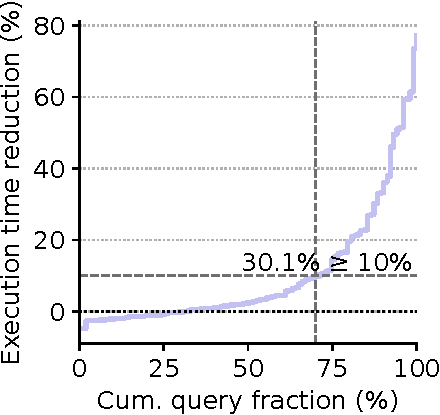
\includegraphics[width=0.245\linewidth]{flexheap/fig/eval/spark/tpcds_vg1_fh.pdf}}
	\subfloat[32 GB]{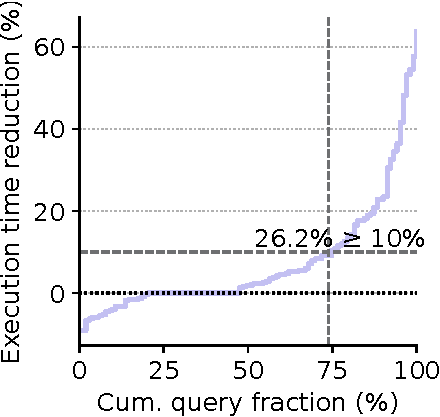
\includegraphics[width=0.245\linewidth]{flexheap/fig/eval/spark/tpcds_vg1_fh_32g.pdf}}
	\subfloat[Q28-VG1]{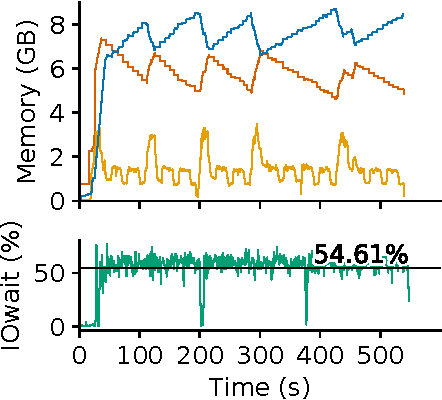
\includegraphics[width=0.245\linewidth]{flexheap/fig/eval/spark/analysis/q28_je_10g_16g.pdf}}
	\subfloat[Q28-FlexHeap]{\includegraphics[width=0.245\linewidth]{flexheap/fig/eval/spark/analysis/q28_fh_10g_16g.pdf}}
	\caption{Performance improvement of \flexheapName{} compared to VG1 in Spark-SQL on TPC-DS.}
	\label{fig:spark_vg1}
\end{figure*}


\subsection{Effects on Tail-Latency for Elasticsearch}

We investigate how the decisions of \flexheapName{} affect the p99 tail-latency of Elasticsearch queries compared to G1 and VG1.
Figure~\ref{fig:es_latency}(a, b) shows the p99 latency of ingestion and search tasks for all the workloads, respectively.

For ingestion tasks, with larger DRAM budgets, \flexheapName{} lowers p99 latency compared to G1-50 because it can grow the heap (up to 90\% of DRAM) when allocation pressure spikes, avoiding queueing and cap-induced full GCs.
On Cohere-Vector, \flexheapName{} reduces p99 by about 10\% compared to G1-50 and by up to 30\% compared to VG1.
VG1’s periodic reclamation rarely triggers during ingestion (the heap is actively used) so its latency typically sits near or slightly above G1’s.
With smaller budgets, \flexheapName{} still reduces p99 by 5--10\% compared to G1, chiefly by cutting GC pressure (in our traces, young/mixed GC counts often drop by about $2\times$) and eliminating cap-driven full GCs.
Moreover, because VG1 keeps the heap near its maximum heap size and leaves less DRAM for the I/O cache, Elasticsearch’s segment flushes during ingestion run against a smaller write-back buffer and take longer.
By preserving more I/O cache, \flexheapName{} reduces flushes and further reducing tail latency.

For search tasks, \flexheapName{} lowers p99 across all DRAM budgets because it reacts to I/O stalls by shrinking the heap and enlarging the I/O cache, which increases cache residency, reduces device read traffic, and shortens queueing at the storage layer.
The effect is strongest with small budgets: on Wikipedia at \SI{8}{GB}, VG1’s p99 is about $1.6\times$ higher than G1 because it keeps the heap near the cap and starves the cache, while \flexheapName{} is about 25\% below G1.
At \SI{12}{GB}, \flexheapName{} remains lower than both mechanisms.
On OpenAI Vector, VG1 sometimes improves latency relative to G1 because it returns memory to the OS more often after the ingestion phase.
\flexheapName{} improves performance further because its shrink decisions consider I/O stalls rather than occupancy targets, resulting in bigger steps of memory release.

\begin{figure*}[h]
	
\includegraphics[width=0.25\linewidth]{flexheap/fig/eval/es_g1_fh_legend.pdf}
	\\
	\subfloat[Ingestion]{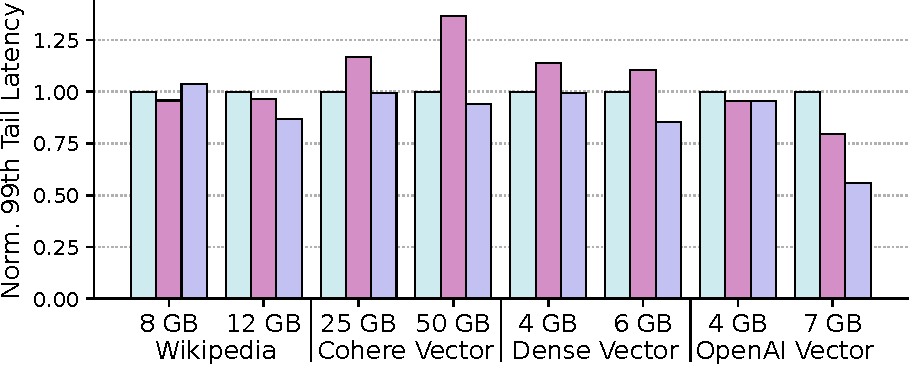
\includegraphics[width=0.495\linewidth]{flexheap/fig/eval/es_ingest_lat.pdf}}
	\subfloat[Search]{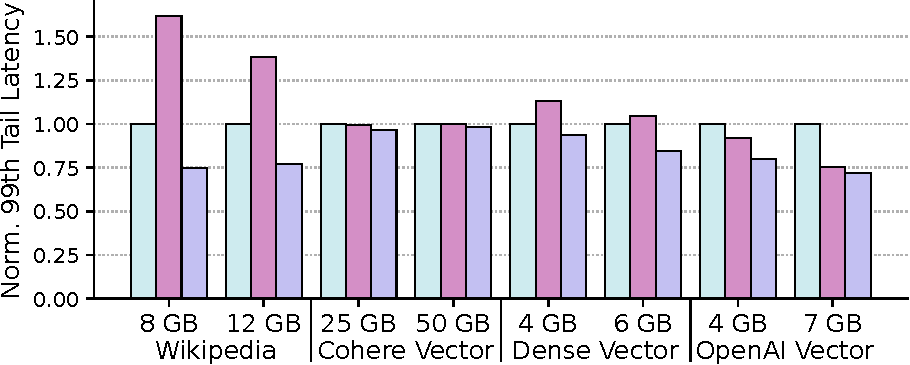
\includegraphics[width=0.495\linewidth]{flexheap/fig/eval/es_search_lat.pdf}}
	\caption{P99 latency of (a) ingestion and (b) search tasks for Elasticsearch
		with G1-50 (maximum heap cap 50\% of DRAM), VG1, and \flexheapName{}.}
	\label{fig:es_latency}
\end{figure*}

\subsection{Sensitivity Analysis}

\paragraph{\textbf{Sensitivity to application phase changes.}}
Here, we investigate how \flexheapName{} adapts to application phases using M1 workload of Lucene.
Compared to G1 (Figure~\ref{fig:phases}(a)), FlexHeap (Figure~\ref{fig:phases}(b)) tracks the application’s five phases much more closely by continuously rebalancing heap and I/O cache memory.
Under G1, the heap quickly grows near its maximum and stays there, pushing the I/O cache down and keeping it low, whereas FlexHeap shrinks and regrows the heap at each phase boundary, leaving several additional gigabytes available in the I/O cache for I/O.
This adaptation shortens multiple phases: the first phase finishes in about 350 s with FlexHeap versus 400 s with G1, and the second phase is dramatically shorter (150 s versus 350 s).
The long final phase is also reduced from roughly 600 s with G1 to about 200 s with FlexHeap.
By maintaining a significantly larger I/O cache and reacting quickly to phase changes, FlexHeap reduces I/O stalls and GC overhead, which directly translates into a substantially lower execution time by 40\%.

\begin{figure*}[h]
	
\includegraphics[width=0.5\linewidth]{flexheap/fig/eval/micro/legend.pdf}
	\\
	\subfloat[G1-90]{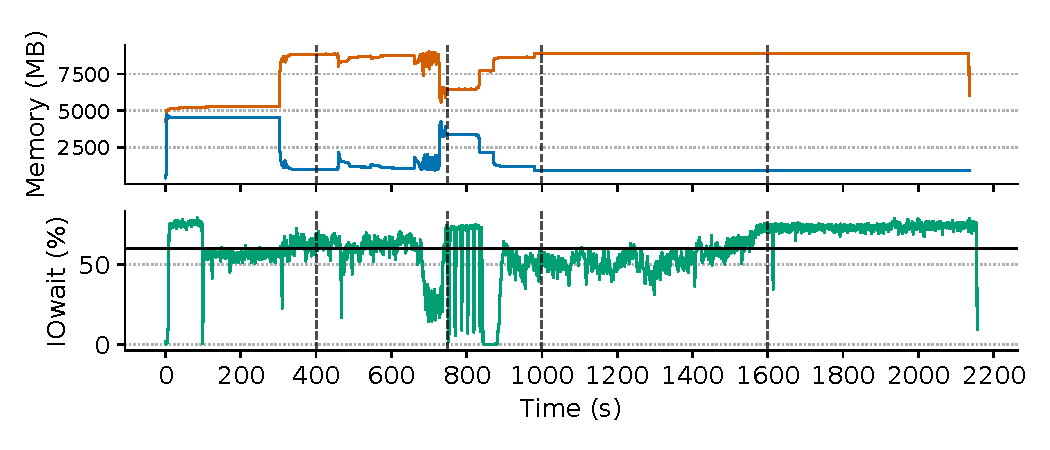
\includegraphics[width=0.495\linewidth]{flexheap/fig/eval/micro/g1_m1.pdf}}
	\subfloat[FlexHeap]{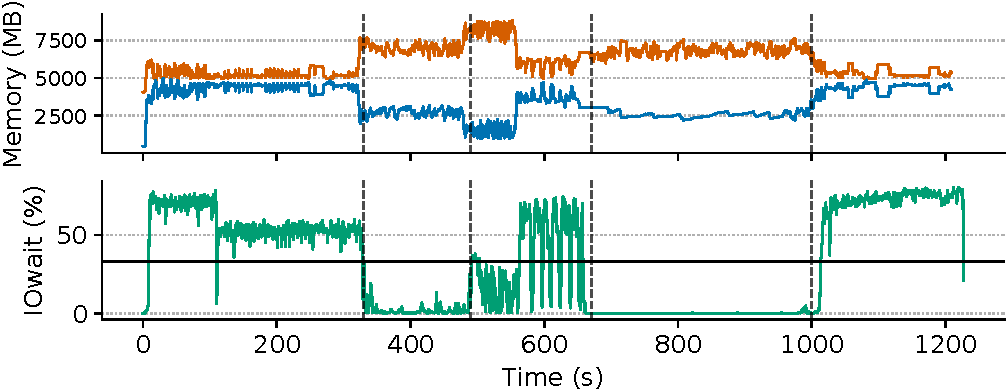
\includegraphics[width=0.495\linewidth]{flexheap/fig/eval/micro/fh_m1.pdf}}
	\caption{Execution of M1 workload over time using (a) G1-90 and (b) \flexheapName{}
		with maximum heap cap 90\% of DRAM budget.}
	\label{fig:phases}
\end{figure*}

\paragraph{\textbf{Sensitivity to device latency.}}
We investigate the benefits of using \flexheapName{} when Lucene utilizes SATA SSDs, which have higher latency than NVMe SSDs but are more cost-effective for storing Lucene's index.
SATA SSDs differ from NVMe SSDs in terms of interface and speed.
NVMe SSDs use the PCIe interface, which provides faster data transfer speed than SATA SSDs that use the older SATA interface.
Also, the read and write throughput of our NVMe SSD is 6$\times$ and 4$\times$ higher compared to SATA SSD, respectively.

\begin{figure}[h]
	\centering
	
\includegraphics[width=0.2\linewidth]{flexheap/fig/eval/sensitivity/lucene_sata_nvme_legend-crop.pdf}
	\hspace{10pt}
	
\includegraphics[width=0.25\linewidth]{flexheap/fig/eval/sensitivity/lucene_breakdowns_legend-crop.pdf}
	\\
	\subfloat[Throughput]{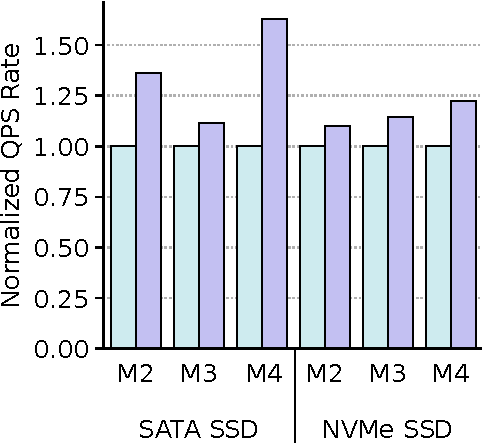
\includegraphics[width=0.25\linewidth]{flexheap/fig/eval/sensitivity/lucene_sata_nvme_qps-crop.pdf}}
	\hspace{10pt}
	\subfloat[GC and IO wait time]{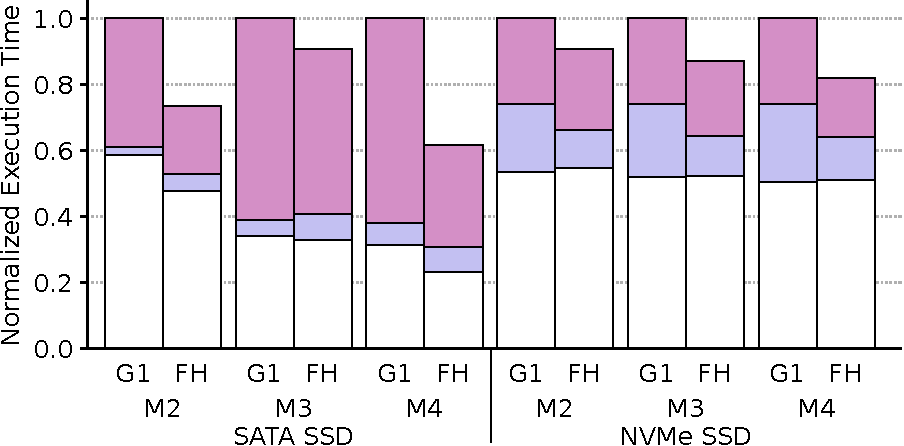
\includegraphics[width=0.45\linewidth]{flexheap/fig/eval/sensitivity/lucene_sata_nvme_breakdowns-crop.pdf}}
	\caption{Lucene (a) throughput and (b) execution time breakdown, comparing G1 and \flexheapName{} (FH) on SATA SSD and NVMe SSD using \SI{5}{GB} DRAM budget.}
	\label{flexheap:fig:sata_ssd}
\end{figure}

Figures~\ref{flexheap:fig:sata_ssd}(a, b) illustrate the throughput and the \flexheapGC{} and I/O wait times for Lucene using SATA SSD and NVMe SSD with a \SI{5}{GB} DRAM budget, respectively.
\flexheapName{} consistently outperforms G1 across all workloads for both types of SSDs.
Notably, the throughput improvement is more pronounced with SATA SSDs, where \flexheapName{} increases throughput by up to 60\% compared to G1, highlighting its effectiveness in environments with higher latency storage.
As shown in Figure~\ref{flexheap:fig:sata_ssd}(b), in experiments with SATA SSD, \flexheapName{} increases \flexheapGC{} time by up to 2.1$\times$ compared to G1 because it prioritizes reducing I/O overhead due to the higher latency of the device.
However, with the reduces latency of NVMe SSDs, the \flexheapGC{} overhead becomes a more significant bottleneck compared to I/O.
Consequently, \flexheapName{} shifts focus to targeting \flexheapGC{} overhead, reducing \flexheapGC{} time by up to 46\% compared to G1.
By dynamically targeting both I/O and \flexheapGC{} overheads, \flexheapName{} adapts effectively to the changing device latency, increasing performance.

\paragraph{\textbf{Sensitivity to resizing step.}}
We evaluate \flexheapName{}’s sensitivity to reallocation step sizes using the M1 workload of Lucene with \SI{5}{GB}, \SI{10}{GB}, \SI{18}{GB}, and \SI{27}{GB} of DRAM (Figure~\ref{fig:reallocation_step}).
The optimal static step varies across DRAM budgets, making offline configuration challenging.
In contrast, the adaptive approach consistently outperforms the best static steps in most cases, with only a 5\% slowdown in the \SI{10}{GB} configuration.
A static 80\% step results in up to $7.7\times$ higher \flexheapGC{} time, highlighting the efficiency of adaptive reallocation.

\begin{figure}[h]
	\centering
	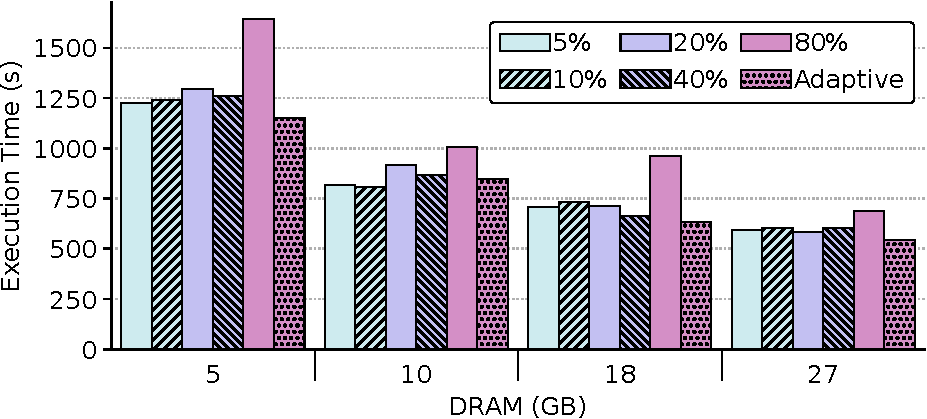
\includegraphics[width=0.5\linewidth]{flexheap/fig/eval/sensitivity/resizing_step-crop.pdf}
	\caption{Execution time of M1 workload in Lucene using static and adaptive reallocation steps for different DRAM budgets.}
	\label{fig:reallocation_step}
\end{figure}
